\documentclass[journal,12pt,twocolumn]{IEEEtran}
%

\usepackage{setspace}
\usepackage{gensymb}
\singlespacing

\usepackage{amsmath}
\usepackage{amsthm}
\usepackage{txfonts}
\usepackage{cite}
\usepackage{enumitem}
\usepackage{mathtools}
\usepackage{listings}
    \usepackage{color}                                            %%
    \usepackage{array}                                            %%
    \usepackage{longtable}                                        %%
    \usepackage{calc}                                             %%
    \usepackage{multirow}                                         %%
    \usepackage{hhline}                                           %%
    \usepackage{ifthen}                                           %%
  %optionally (for landscape tables embedded in another document): %%
    \usepackage{lscape}     
\usepackage{multicol}
\usepackage{chngcntr}
\renewcommand\thesection{\arabic{section}}
\renewcommand\thesubsection{\thesection.\arabic{subsection}}
\renewcommand\thesubsubsection{\thesubsection.\arabic{subsubsection}}

% correct bad hyphenation here
\hyphenation{op-tical net-works semi-conduc-tor}
\def\inputGnumericTable{}                                 %%

\lstset{
%language=C,
frame=single, 
breaklines=true,
columns=fullflexible
}

\begin{document}
%


\newtheorem{theorem}{Theorem}[section]
\newtheorem{problem}{Problem}
\newtheorem{proposition}{Proposition}[section]
\newtheorem{lemma}{Lemma}[section]
\newtheorem{corollary}[theorem]{Corollary}
\newtheorem{example}{Example}[section]
\newtheorem{definition}[problem]{Definition}
\newcommand{\BEQA}{\begin{eqnarray}}
\newcommand{\EEQA}{\end{eqnarray}}
\newcommand{\define}{\stackrel{\triangle}{=}}

\bibliographystyle{IEEEtran}


\providecommand{\mbf}{\mathbf}
\providecommand{\pr}[1]{\ensuremath{\Pr\left(#1\right)}}
\providecommand{\qfunc}[1]{\ensuremath{Q\left(#1\right)}}
\providecommand{\sbrak}[1]{\ensuremath{{}\left[#1\right]}}
\providecommand{\lsbrak}[1]{\ensuremath{{}\left[#1\right.}}
\providecommand{\rsbrak}[1]{\ensuremath{{}\left.#1\right]}}
\providecommand{\brak}[1]{\ensuremath{\left(#1\right)}}
\providecommand{\lbrak}[1]{\ensuremath{\left(#1\right.}}
\providecommand{\rbrak}[1]{\ensuremath{\left.#1\right)}}
\providecommand{\cbrak}[1]{\ensuremath{\left\{#1\right\}}}
\providecommand{\lcbrak}[1]{\ensuremath{\left\{#1\right.}}
\providecommand{\rcbrak}[1]{\ensuremath{\left.#1\right\}}}
\theoremstyle{remark}
\newtheorem{rem}{Remark}
\newcommand{\sgn}{\mathop{\mathrm{sgn}}}
\providecommand{\abs}[1]{\lvert#1\rvert}
\providecommand{\res}[1]{\Res\displaylimits_{#1}} 
\providecommand{\norm}[1]{\lVert#1\rVert}
\providecommand{\mtx}[1]{\mathbf{#1}}
% \providecommand{\mean}[1]{E\left[ #1 \right]}
\providecommand{\fourier}{\overset{\mathcal{F}}{ \rightleftharpoons}}
\providecommand{\system}{\overset{\mathcal{H}}{ \longleftrightarrow}}
\newcommand{\solution}{\noindent \textbf{Solution: }}
\newcommand{\cosec}{\,\text{cosec}\,}
\providecommand{\dec}[2]{\ensuremath{\overset{#1}{\underset{#2}{\gtrless}}}}
\newcommand{\myvec}[1]{\ensuremath{\begin{pmatrix}#1\end{pmatrix}}}
\newcommand{\cmyvec}[1]{\ensuremath{\begin{pmatrix*}[c]#1\end{pmatrix*}}}
\newcommand{\mydet}[1]{\ensuremath{\begin{vmatrix}#1\end{vmatrix}}}
\newcommand{\proj}[2]{\textbf{proj}_{\vec{#1}}\vec{#2}}
\newcommand{\RNum}[1]{\uppercase\expandafter{\romannumeral #1\relax}}
\let\StandardTheFigure\thefigure
\let\vec\mathbf


\title{
\LARGE SM5083\\
    \LARGE Assignment Number 2 \\[0.5em]
    
    \large Deevanshu M.Gupta\par
    \large   SM21MTECH12014  \par
}
\maketitle


\renewcommand{\thefigure}{\theenumi}
\renewcommand{\thetable}{\theenumi}




\section{ chapter \RNum{3} Miscellaneous Examples \RNum{6} Q.17 }


\textbf{1. From a point P(h,k) are drawn perpendicular to the axes, prove that the length of the line that joins the feet of the perpendicular is $ sin\omega \sqrt{h^2+k^2+2hkcos\omega }$.
\newline Note: The angle between the axes is $\omega $}

\solution

let
OX and OY be the axis, P be the point (h,k), PK and PH be the perpendicular on the OX and OY respectively.
\newline draw a parallel line of OY from P to A in line OX such that the length of OA is h and $\angle PAK =  \omega $
\newline similarly, draw a parallel line of OX from P to B in line OY such that the length of OB is k and $\angle PBH = \omega $
\newline From the figure,\ref{fig:assignment02}
\begin{align}
    OK = h + k cos\omega \\ ~\text{and}~
    OH = k + h cos\omega 
\end{align}
\begin{align}
 \\ \therefore
HK^2 = OK^2 + OH^2 -2(OK)(OH) cos\omega\\
HK^2 = ( h + k cos\omega)^2 + ( k + h cos\omega)^2 \\ 
 -2(h + k cos\omega )( k + h cos\omega) cos\omega \nonumber \\
 \newline\text{by putting,} cos^2\omega = 1 - sin^2\omega \nonumber
\\HK^2 = (h^2 + k^2)(sin^2\omega) + 2khcos\omega(sin^2\omega)
\end{align}
\begin{figure}[!ht]
	\centering
	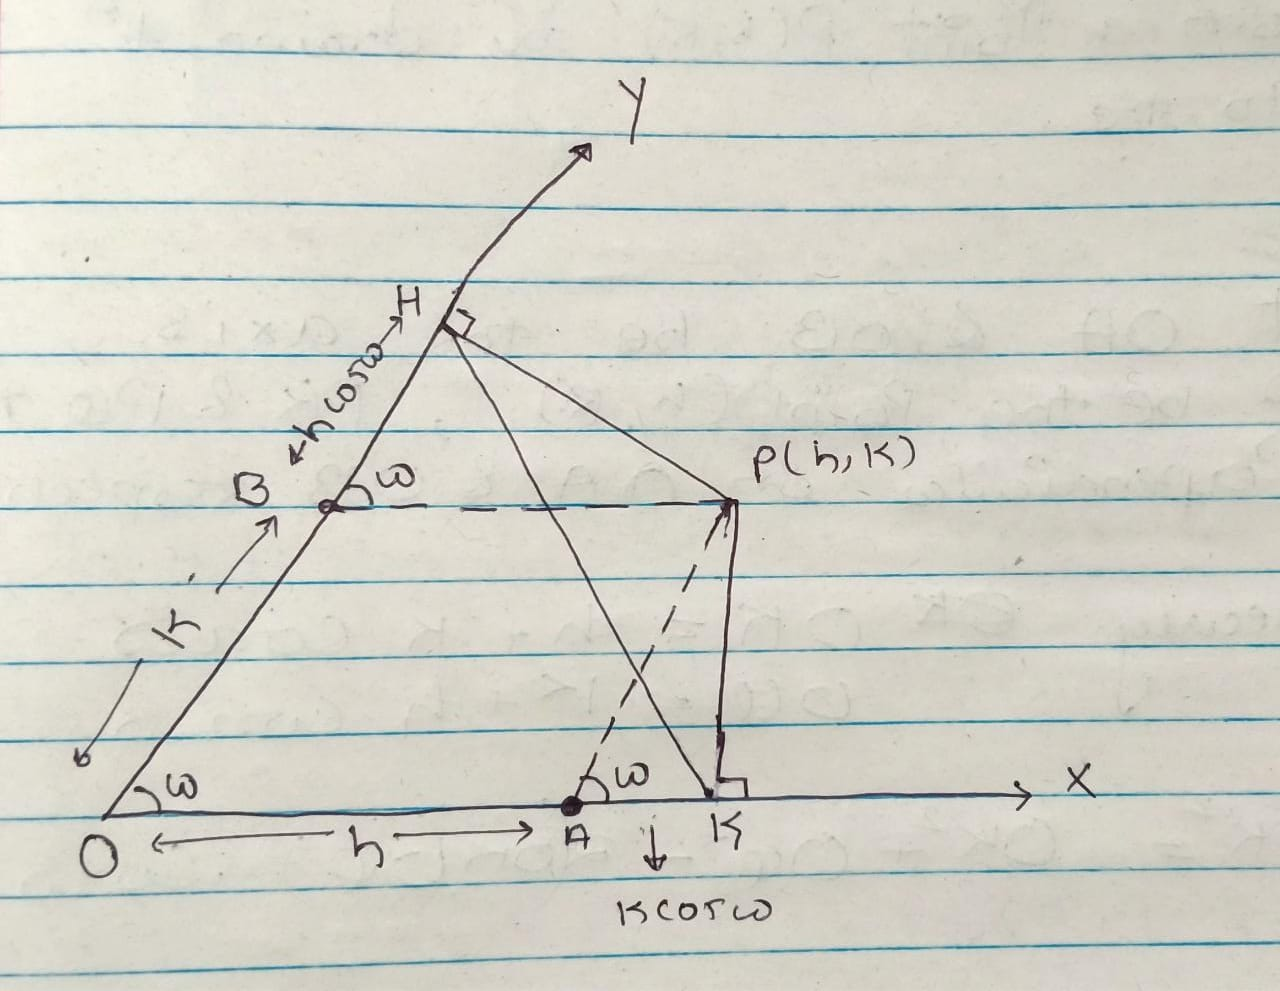
\includegraphics[width=\columnwidth]{assignment2.jpeg}
	\caption{Rough figure for our question}
	\label{fig:assignment02}
\end{figure}

\begin{align}
  HK =  sin\omega \sqrt{h^2+k^2+2hkcos\omega }
\end{align}


    
    



\end{document}


